\section{Anotación}

Hasta este momento describimos la recolección de los datos, a lo cual le siguió la selección de los artículos y comentarios a anotar. Pasamos ahora a detallar el último paso de la construcción del conjunto de datos: el etiquetado. En primer lugar, adoptamos nuestra propia definición de discurso de odio, con la cual confeccionamos el respectivo manual de etiquetado. Con esto en mano, definimos las variables que nos interesa anotar sobre los datos. Llamamos a esto \emph{modelo de etiquetado} \cite{pustejovsky2012natural}.

Finalmente, especificamos el proceso concreto de etiquetado. Por un lado, la selección de anotadores, sus perfiles y la herramienta de etiquetado. Por el otro, el esquema utilizado para distribuir el trabajo a los anotadores.

\todo{Agregar en algún lado Data Statements}


\subsection{Definición de discurso de odio y manual de etiquetado}
\label{sec:05_hate_speech_definition}
\begin{table}[b]
    \centering
    \small
    \begin{tabular}{p{0.2\textwidth} p{0.6\textwidth}}
        Nombre & Descripción \\
        \hline
        MUJER        & Misoginia, agresiones basadas en ser mujer  \\
        LGBTI        & Homofobia, transfobia, y ofensas a la comunidad LGBTI \\
        RACISMO      & Racismo, Xenofobia, Judeofobia, etc \\
        POBREZA      & Basado en su condición de clase \\
        POLITICA     & En base a la filiación política del agredido \\
        ASPECTO      & Gordofobia, gerontofobia \\
        CRIMINAL     & Criminales, presos, y personas en conflicto con la ley \\
        DISCAPACIDAD & Discapacidades y problemas de adicciones \\
        \hline
    \end{tabular}
    \caption{Características protegidas consideradas en este trabajo. Consideramos una agrupación de ciertas características bajo una misma denominación: por ejemplo, LGBTI contempla homofobia, transfobia, entre otras; análogamente racismo puede contemplar xenofobia, y otras variantes de este fenómeno. }
    \label{tab:caracteristicas_protegidas}
\end{table}


Teniendo en cuenta las consideraciones de la Sección \ref{sec:hate_speech_definitions}, elaboramos nuestra propia definición de discurso de odio. Entendemos que hay discurso de odio en un comentario de una red social si éste contiene declaraciones de carácter intenso e irracional de rechazo, enemistad y aborrecimiento contra un individuo o contra un grupo de personas por poseer (o aparentar poseer) una característica protegida \footnote{Ver Sección \ref{sec:hate_speech_definitions} para la definición de característica protegida}. Esta expresión puede manifestarse de manera explícita como insultos directos, celebraciones de crímenes, incitaciones a tomar medidas contra el individuo o grupo, o también expresiones más veladas, por ejemplo de contenido irónico. Consideramos en esta definición que no es suficiente un insulto o una agresión para que se configure discurso de odio: es necesario hacer una apelación explícita o implícita al menos a una característica protegida.

A diferencia de otros trabajos, nuestra definición comprende varias características, incluso algunas que están en la frontera de ser protegidas. Los estudios previos que hemos listado en la Sección \ref{sec:hate_speech_previous_work} han estado centrados mayormente en racismo y misoginia, con algunos que han agregado homofobia. En nuestra definición comprenderemos --además de la misoginia y el racismo-- a la homofobia y transfobia; al odio de clase (a veces conocido como aporofobia); al odio por aspecto físico; a la discriminación por discapacidad o problemas de salud; entre otras. En particular, hay dos características no convencionales que tuvimos en cuenta. En primer lugar, consideramos el \tbf{discurso de odio político}, que, de acuerdo a la CIDH \cite{CIDH2015}, es difícil considerar como protegido ya que puede dar lugar a censura y restricciones a la libertad de expresión. Por otro lado, consideramos el \tbf{discurso de odio contra criminales}, presos, y otras personas en situación de conflicto con la ley. Si bien este punto ni siquiera es considerado como protegido en ninguno de los tratados mencionados en la Sección \ref{sec:hate_speech_definitions}, agregamos esta característica debido a la enorme cantidad de contenido alentando la violencia contra criminales en las noticias policiales. Teniendo en cuenta que nos interesa detectar particularmente incitaciones a realizar acciones violentas contra individuos o grupos, relajamos nuestra definición para incluir esta clase de agresiones.

Tenemos entonces ocho características que agrupan distintos tipos de discurso de odio: contra las mujeres; racismo y xenofobia; contra la comunidad LGBTI; odio de clase; gordofobia, gerontofobia y demás discurso de odio por aspecto; por su ideología política; contra criminales; y finalmente contra discapacitados y adictos. Las características en cuestión son listadas en la Tabla \ref{tab:caracteristicas_protegidas} junto a nombres de referencia que serán usados en éste y el próximo capítulo.

Con esta definición confeccionamos un manual de referencia para los anotadores. Tanto el manual como la definición fueron desarrollados iterativamente, primero realizando algunas pruebas de etiquetado entre miembros del equipo y rondas de discusión posteriores analizando los ejemplos problemáticos y casos borde. De estas iteraciones logramos ir mejorando la definición y el manual hasta llegar a una versión definitiva. Para cada característica agregamos consideraciones adicionales sobre lo que pensamos que configura discurso de odio: por ejemplo, para la característica MUJER no es suficiente con que un insulto sino que es necesario se apele a algo distintivo de la mujer (``algo que no le diría a un hombre''); para la característica LGBTI incluimos particularmente las expresiones de asco, y puntualmente a los emojis que representen esto. En el Apéndice \ref{app:manual_criterios_anotacion} puede encontrarse el manual de etiquetado completo entregado a los etiquetadores.



\subsection{Modelo de etiquetado}
\label{sec:modelo_etiquetado}

\begin{figure}[t]
    \centering
    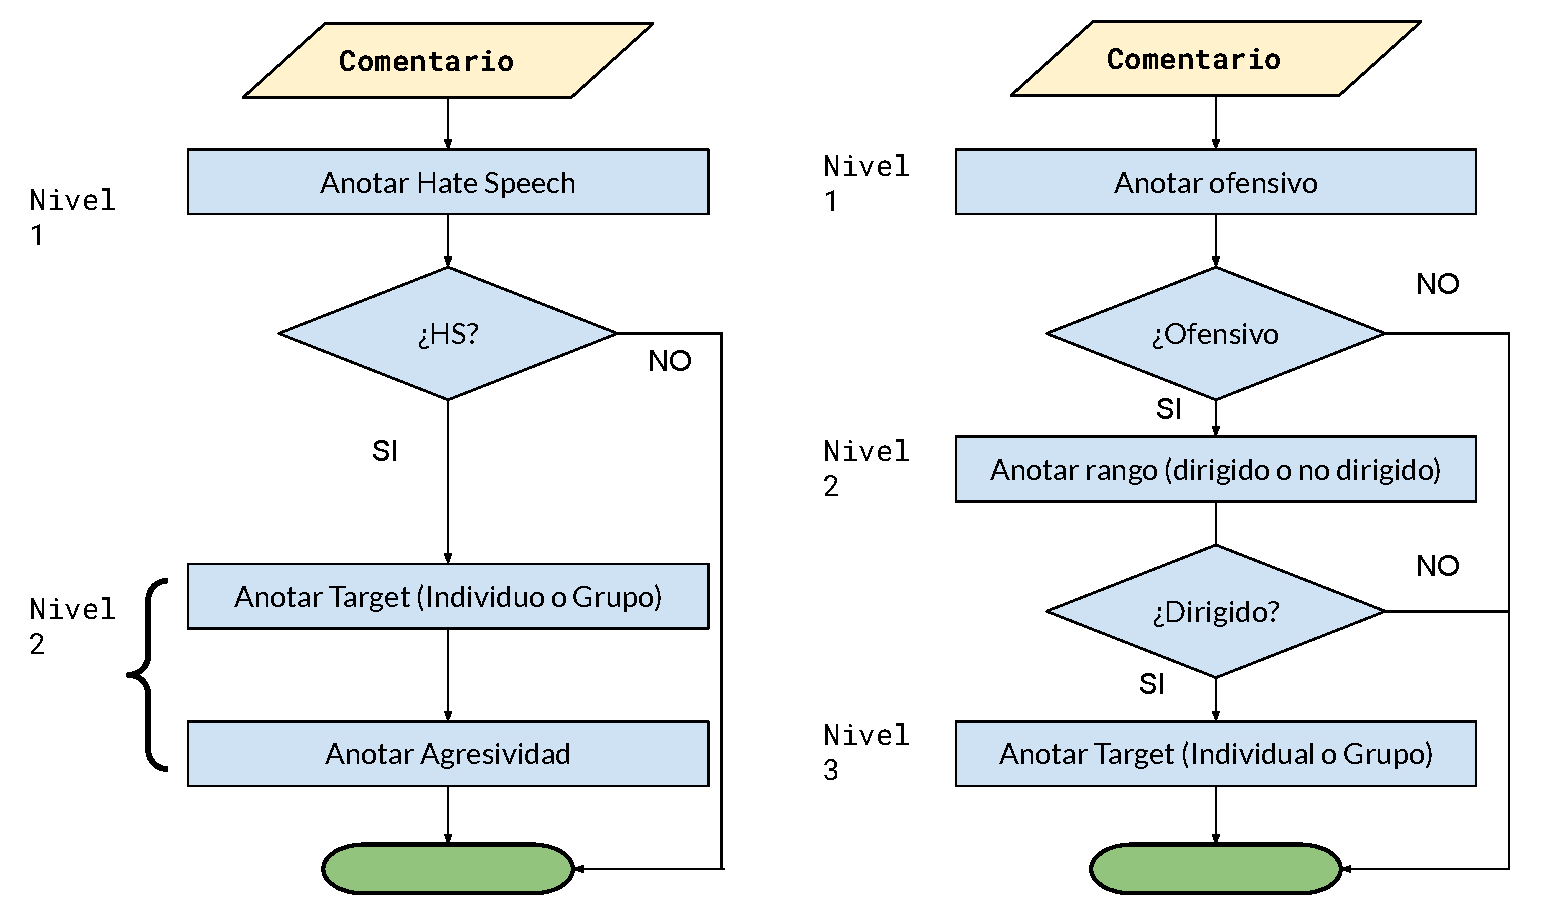
\includegraphics[width=\textwidth]{img/05/modelos_jerarquicos.pdf}
    \caption{Modelos jerárquicos de anotación. A la izquierda, tenemos el modelo jerárquico propuesto para HatEval \cite{hateval2019semeval}, a la derecha el modelo propuesto para OffensEval \cite{zampieri2019semeval2019}}
    \label{fig:modelos_offenseval_hateval}
\end{figure}


Un modelo de anotación es una representación práctica del objetivo de este proceso; es decir, del fenómeno que queremos capturar \cite{pustejovsky2012natural}. En base a la discusión del capítulo anterior, es de interés marcar comentarios discriminatorios de manera granular de modo de tener información de qué grupos y/o características se está ofendiendo. Para identificar formas más graves de discurso de odio, también es de interés identificar llamados a tomar alguna acción (violenta o no violenta) contra esa persona o grupo.

\citet{zampieri2019predicting} introdujeron un modelo jerárquico de anotación para la tarea de lenguaje ofensivo, utilizado tanto en los datasets de OffensEval \cite{zampieri2019semeval2019} y HatEval \cite{hateval2019semeval}. La idea de este modelo es realizar anotaciones en varios niveles, sólo marcando algunas variables de acuerdo a las respuestas del nivel anterior. Por ejemplo, en el caso de \hateval{}, tenemos un primer nivel que consta de marcar si un tweet contiene o no discurso de odio. Si el tweet tiene discurso de odio, entonces se anota en primer lugar si está dirigido a un individuo o a un grupo, y también si es agresivo o no. En el caso de \emph{OffensEval}, primero se anota si es ofensivo, y en caso de serlo, se marca si está dirigido a un individuo o grupo o es un insulto no dirigido. Por último, si es dirigido y ofensivo, marcamos si su objetivo es un grupo o un individuo. La Figura \ref{fig:modelos_offenseval_hateval} ilustra en modo de diagrama de flujo el modelo de anotación de ambos conjuntos de datos.


%
%
% Link: https://docs.google.com/drawings/d/14TKSC4QmZhksnlFvQcHUaZup-q3AL0Up1cNKJUr5toI/edit
%



\begin{figure}[t]
    \centering
    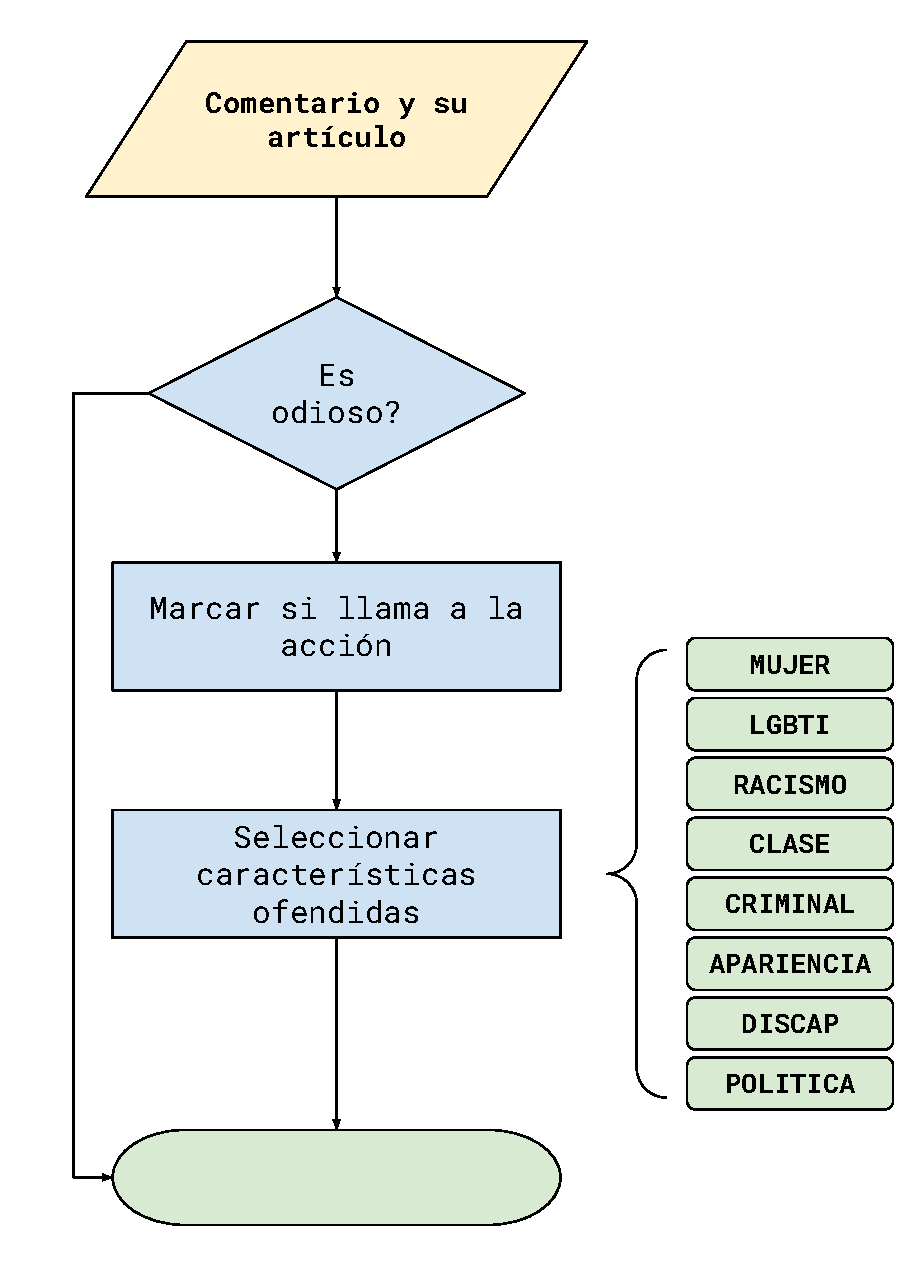
\includegraphics[width=0.5\textwidth]{img/05/annotation_model.pdf}
    \caption{Modelo de anotación para el dataset construido en este capítulo. El modelo jerárquico consta de dos niveles: el primero, donde se anota si es odioso. El segundo consta de anotar --en caso de haber sido marcado como odioso-- si contiene un llamado a la acción y a qué características ofende.}
    \label{fig:annotation_model}
\end{figure}


Basándonos en esta estructura jerárquica planteamos nuestro modelo, ilustrado en la Figura \ref{fig:annotation_model}. Para cada comentario y su respectivo contexto (el artículo), requerimos una anotación para decidir si el comentario es odioso o no. Si no es odioso, no se necesita más información. En caso de haberse marcado como odioso, el par artículo-comentario debe contener, además, una anotación por si llama o no a la acción, y al menos una categoría protegida marcada como ofendida.


\subsection{Etiquetadores}

%
% Chequear https://docs.google.com/spreadsheets/d/1PaOVw_tKVRvjZIqRl2YKnaNsvX5tHJjjY0CV9PLrc6g/edit?resourcekey#gid=366330815
%

\begin{table}[b]
    \centering
    \small
    \begin{tabularx}{\textwidth}{l l l l l l l l}
        Género& Edad  & Estudios    & Área          & Identificación    & ¿Activista?   & Experiencia\\
        \hline
        F    & 25-30  & Doctorado*  & Psicología    & Mujer             & No                   & Sí         \\
        NB   & 30-35  & Grado*      & Artes         & LGBTI             & No                   & No         \\
        F    & 30-35  & Grado*      & Antropología  & Mujer, LGBTI      & Feminista            & Sí         \\
        M    & 35-40  & Grado       & Sociología    & No                & No                   & No         \\
        F    & 35-40  & Doctorado   & Psicología    & Mujer             & No                   & No         \\
        F    & 30-35  & Grado       & Comunicación  & No                & Migrantes            & No         \\
        \hline
    \end{tabularx}
    \caption{Información sobre los anotadores. En el caso de estudios, * indica en curso. Indentificación se refiere a si se autopercibe como perteneciente de una característica protegida considerada en este trabajo. Experiencia se refiere a haber etiquetado previamente otros conjuntos de datos. }
    \label{tab:informacion_sobre_anotadores}
\end{table}

A diferencia de otros trabajos de detección de discurso de odio, decidimos garantizar que nuestros anotadores estuvieran más cerca culturalmente al problema en cuestión. El discurso de odio tiene un fuerte componente cultural, muchas veces expresado a través de jerga o expresiones dialectales muy particulares, y está relacionado con noticias muy propias de esta región. Es por esto que decidimos buscar por nuestros propios medios perfiles alineados a estos puntos y no depender de plataformas externas de crowdsourcing para esta tarea.

Reclutamos etiquetadores hablantes nativos de español rioplatense, estudiantes o graduados/as de carreras de ciencias sociales, humanidades o afines -- como ser Psicología, Sociología, Comunicación, Artes, Antropología. Para evitar sesgos en la tarea, nos interesó que no tuvieran conocimientos de inteligencia artificial o ciencia de datos. Por último, también fue de interés que sean usuarios asiduos de redes sociales para poder captar las sutilezas del lenguaje en ese medio.

El proceso de reclutamiento constó de una breve entrevista donde corroboramos que los etiquetadores fueran hablantes nativos de español rioplatense, a la vez que les describimos la tarea que debían realizar y la herramienta correspondiente de etiquetado. Luego de la entrevista, se les solicitó hacer una prueba paga que constó de leer el manual de etiquetado y anotar 10 artículos. Esto fue realizado para corroborar la calidad de los etiquetadores, aunque no rechazamos ningún postulante en este proceso. La Tabla \ref{tab:informacion_sobre_anotadores} brinda información desagregada sobre los seis etiquetadores contratados para la tarea. Los etiquetadores reclutados tienen un perfil altamente escolarizado, y dos de quienes contratamos con experiencia previa en la tarea de anotación. Un punto adicional a marcar es que dos de las etiquetadoras eran activistas --al momento de realizarse el estudio-- en organizaciones relacionadas a alguno de los grupos vulnerados que estudiamos en este trabajo.

Luego de la entrevista, se les dio una devolución de su anotación y se les reasignaron cinco de los artículos seleccionados junto a diez más (15 en total) para su anotación a modo de entrenamiento. Este fue el único conjunto de artículos que fue anotado por la totalidad de los anotadores. Al finalizar esta etapa, se les brindó una nueva devolución para ajustar el criterio de anotación, y se procedió a la etapa de anotación del dataset.

\subsection{Esquema de anotación}


%%
%%
%% Link a Google Draw:
%% https://docs.google.com/drawings/d/1esS9tAwpPVydohxd-B-xwVdAaPQRVGAo0MruBrgSKig/edit
%%
%%

\begin{figure}
    \centering
    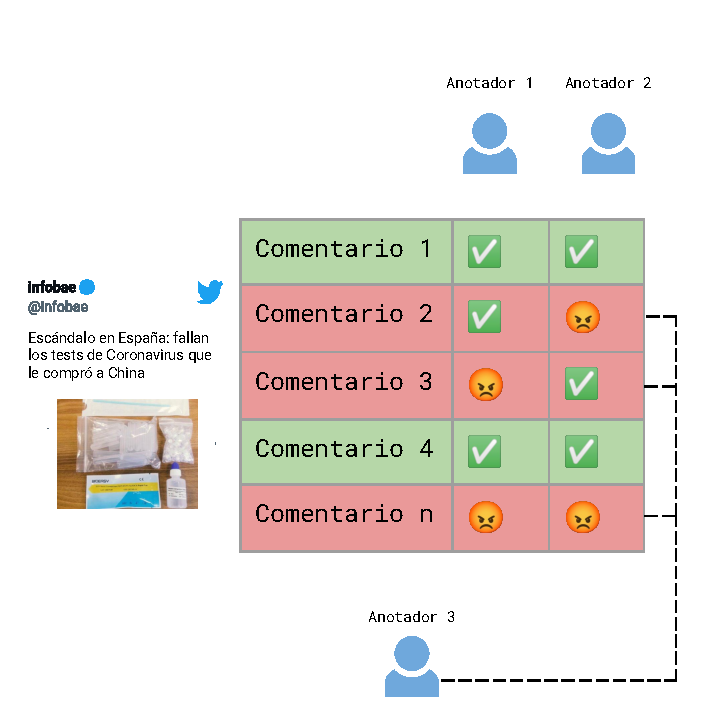
\includegraphics[width=\textwidth]{img/05/esquema_anotacion.pdf}
    \caption{Esquema de anotación. Caso en que ambos anotadores etiqueten los comentarios del artículo}
    \label{fig:annotation_schema}
\end{figure}

Pasamos ahora a describir la mecánica del proceso de anotación. Para lo que respecta a este trabajo, tomamos como la unidad de anotación al artículo. Cada etiquetador, al serle presentado un artículo, tuvo dos opciones: etiquetarlo o saltearlo. En caso de decidir etiquetarlo, tuvo que marcar las etiquetas correspondientes a cada uno de los comentarios del artículo de acuerdo al modelo descripto. La idea de permitir el salteado fue doble: evitar contenido poco interesante en términos de comentarios discriminatorios, y también dar la posibilidad al trabajador de evitar contenido sensible o perturbador para su persona.

Considerando la dificultad de la tarea y los límites borrosos del discurso de odio, decidimos seguir un esquema de etiquetado similar al de trabajos previos donde múltiples personas anotan una misma instancia. Una posibilidad considerada en un principio fue asignar el artículo completo a tres anotadores; sin embargo, esta modalidad sería ineficiente dada la baja cantidad de contenido discriminatorio observada preliminarmente entre los comentarios seleccionados. Decidimos entonces ir por un esquema de desempate similar al de \citet{hateval2019semeval}: dos personas anotan un artículo, y luego un tercero anota sólo aquellos comentarios donde al menos uno marcó que existe contenido odioso. Esta modalidad permite que haya una tercera anotación incluso cuando las dos previas marcaron contenido odioso, siendo esto realizado para recolectar más información sobre los comentarios. Dada la incidencia de comentarios odiosos (que veremos luego en los resultados) la adición de esta tercera etiqueta en estos casos técnicamente innecesarios tuvo un bajo costo.



%%
%%
%% Link a Google Draw
%% https://docs.google.com/drawings/d/1TOlCgZggCmYHgZWV7ZrIIlXuhcFUMeYw4PcFM7XdY2k/edit
%%
%%

\begin{figure}
    \centering
    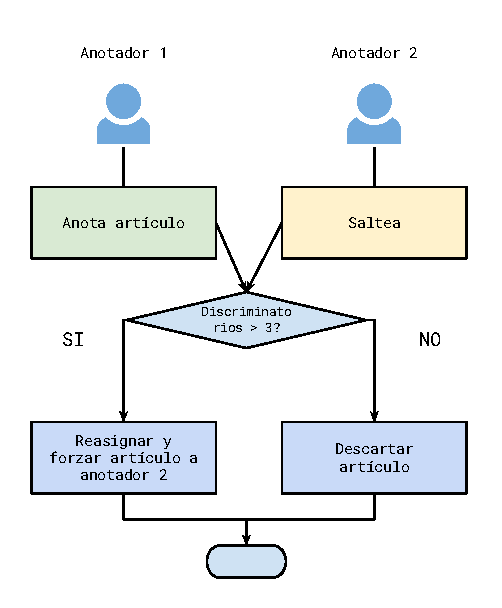
\includegraphics[width=0.5\textwidth]{img/esquema_anotacion_caso_2.pdf}
    \caption{Esquema de anotación. Caso en que un anotador decida saltear}
    \label{fig:annotation_schema_case_two}
\end{figure}


La Figura \ref{fig:annotation_schema} ilustra el flujo en el caso de que ninguno de los anotadores asignados decida saltear el artículo. Ahora ¿qué pasa si alguno de los dos anotadores decide saltear el artículo?

\begin{enumerate}
    \item Si los dos etiquetadores asignados deciden pasar por alto el artículo asignado, entonces lo descartamos del conjunto de datos
    \item En el caso de que uno lo saltee y el otro lo anote y encuentre menos de 4 comentarios odiosos, entonces también descartamos el artículo
    \item En el caso de que uno lo saltee y el otro lo anote encontrando cuatro o más comentarios odiosos, entonces reasignamos el artículo al etiquetador que salteó, sin darle esta vez posibilidad a que no lo anote
\end{enumerate}

Tomamos la decisión de descartar los artículos en los dos primeros casos intentando maximizar la tasa de comentarios discriminatorios encontrados. En caso de reasignar el artículo, revocamos la posibilidad de saltearlo \footnote{Teniendo en cuenta la posibilidad de que hayan salteado por contenido perturbador para el anotador, dimos la posibilidad de que nos avisen que no querían trabajar en ese artículo. No hubo problemas al respecto de todas formas}. La Figura \ref{fig:annotation_schema_case_two} ilustra el esquema de anotación de artículos recién descripto, que se complementa con el de la Figura \ref{fig:annotation_schema}.



%Con este esquema, y teniendo en cuenta los números finales obtenidos del dataset, dedicamos 2.16 etiquetados por comentarios versus 3 etiquetados por comentario de anotar tres veces todo.


Como resultado de este esquema, cada comentario de nuestro dataset puede tener dos o tres anotaciones, siendo los casos posibles los siguientes:

\begin{enumerate}
    \item Dos anotaciones negativas: es decir, que no encuentran discurso de odio en el comentario
    \item Tres anotaciones, con al menos una que marque el comentario como odioso
\end{enumerate}


%
% Esto quizás va después
%
\subsection{Herramienta de etiquetado}

%%
%% Link a Google Draw: https://docs.google.com/drawings/d/1E24-2l6hsNj2JSKBZOD8QvZCJR6rrGjz-cWwt8XuPRg/edit
%%

\begin{figure}
    \centering
    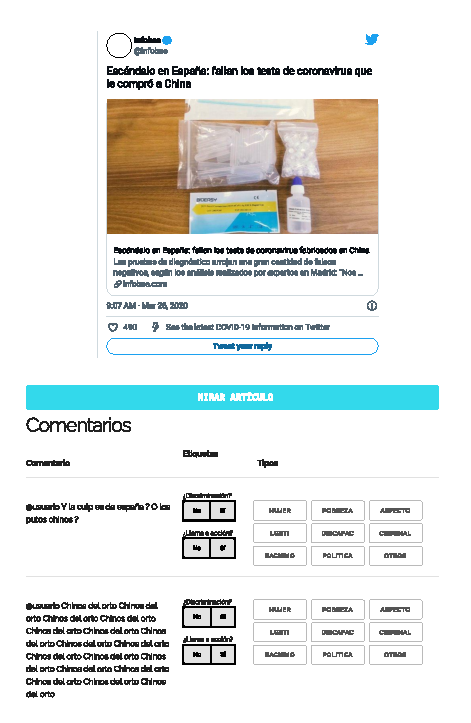
\includegraphics[width=\textwidth]{img/labeler.pdf}
    \caption{Pantalla del etiquetador}
    \label{fig:labeler_example}
\end{figure}

Al no optar por utilizar servicios de etiquetado tercerizado, desarrollamos nuestra propia aplicación para esta tarea. Cada etiquetador tuvo acceso a un sitio web donde se le mostraron uno a uno los artículos asignados, de acuerdo al orden establecido por los administradores de la aplicación. La Figura \ref{fig:labeler_example} ilustra la interfaz de anotación presentada a los usuarios del sistema. Cada artículo es presentado junto a su tweet correspondiente, al texto replegado de la noticia --en caso de que un usuario requiera su lectura-- y a los comentarios.

Ante esto, el etiquetador puede elegir saltear el artículo o etiquetarlo. Si decide etiquetarlo, debe para cada comentario marcar usando un control de tipo interruptor:

\begin{enumerate}
    \item Si el comentario contiene discurso discriminatorio.
    \item En caso de ser discriminatorio, marcar si llama a la acción.
    \item En caso de ser discriminatorio, marcar al menos una característica ofendida.
\end{enumerate}

Para el desarrollo de la aplicación usamos \emph{Django} \footnote{\url{https://www.djangoproject.com/}}, un framework de Python para desarrollo web, y Javascript plano. Como base de datos utilizamos \emph{SQLite}, ya que el sistema no tuvo grandes requerimientos de concurrencia (sólo seis o siete usuarios simultáneos).


Cada tweet fue presentado con un preprocesado básico que consistió en reemplazar handles de usuarios por un token especial \verb|@usuario| para evitar cualquier sesgo. Por ejemplo, si un usuario A conocido como difusor de discurso discriminatorio retwittea la noticia y otro responde a ese retweet, en el tweet aparece el nombre de A, lo cual podría condicionar a quien tenga que evaluar ese comentario.


\subsection{Asignación}

Llamamos \tbf{asignación} al procedimiento de colocar \tbf{etiquetas} (también llamadas \emph{gold labels}) a las instancias de nuestro conjunto de datos \cite{pustejovsky2012natural}. El modelo descripto en la Sección \ref{sec:modelo_etiquetado} consta de una etiqueta binaria que marca si el contenido es discriminatorio o no (notamos HS) en el primer nivel, y luego 9 etiquetas binarias para el segundo: una para las llamadas a la acción (notamos CALLS) y otras ocho para las características ofendidas listadas en la Tabla \ref{tab:caracteristicas_protegidas}. Recordemos que una anotación negativa sólo consta de HS negativo, mientras que una positiva consta de un HS positivo, una etiqueta para CALLS y al menos una etiqueta positiva de las características ofendidas.

Pensamos el proceso de asignación de etiquetas como una votación, donde cada anotador da un voto para cada variable a asignar. Detallamos a continuación cómo fueron asignadas las etiquetas del conjunto de datos:

\begin{enumerate}
    \item Para la etiqueta de HS, asignamos mediante votación mayoritaria: 2 o más votos para HS positivo, caso contrario HS negativo.
    \item En caso de haber marcado que hay HS: marcamos CALLS es positivo por votación mayoritaria.
    \item En caso de haber marcado que hay HS: marcamos como positivas todas aquellas características marcadas por los anotadores.
\end{enumerate}

La primer decisión es la más obvia y razonable: para que un comentario sea considerado como odioso (HS positivo) tiene que ocurrir que al menos dos etiquetadores lo marquen como tal. Si se anota HS positivo, para que CALLS sea positivo tiene que haber al menos dos votos en tal sentido. Si un anotador marcó que hay llamado a la acción y otro que no, asignamos CALLS negativo. \todo{Acá Agus pregunta por qué no asignamos CALLS si al menos uno marca. Me parece que no es la idea: corresponde que haya cierto consenso sobre que está dado este fenómeno. Con el mismo criterio, deberíamos marcar así HS}

En el caso de las características no realizamos votación mayoritaria, sino que la anotamos si al menos un etiquetador lo hizo. Esta decisión podría haberse tomado de otra manera; por ejemplo, sólo tomando aquellos casos donde haya cierto grado de coincidencia entre los comentarios. Sin embargo, al considerar que los límites entre las características son difusos (por ejemplo, APARIENCIA y MUJER tienen una intersección no nula y a veces CLASE y RACISMO también) preferimos anotarlas de esta manera.
